\chapter { پیاده سازی }

در این بخش به روش‌ها و ابزارهای استفاده شده در پیاده‌سازی سیستم انیمیشن اشاره خواهد شد

\section {ابزارها}

\subsection {
    \lr{OpenGL}
    }

\lr{OpenGL}
یک واسط برنامه نویسی کاربردی  
\LTRfootnote{API}
است که با فراهم کردن توابع زیادی به توسعه‌دهندگان امکان دستکاری گرافیک و تصاویر را می‌دهد.
\lr{OpenGL} 
یک کتابخانه‌ی رندرینگ است.
یک "شئ" به خودی خود در
\lr{OpenGL} 
مفهومی ندارد
و به صورت مجموعه‌ای از مثلث‌ها و حالات مختلف درنظر گرفته می‌شود. بنابراین  
وظیفه‌ی ما است که بدانیم چه شئ‌ای در کدام قسمت صفحه رندر شده است. این کتابخانه تنها وظیفه‌اش کشیدن تصاویری که است که می‌خواهیم به تصویر کشیده‌شوند.
در این صورت اگر می‌خواهیم تصویری را به‌روزرسانی کنیم و یا به عنوان مثال شئ‌ای را تحرک دهیم باید به 
\lr{OpenGL}
درخواست دهیم که صحنه را دوباره‌برای ما رندر کند.
\cite{KhronosUsingOpenGL}

به صورت کلی 
\lr{OpenGL}
را می‌توان یک ماشین حالت بزرگ درنظر گرفت. هر حالت شامل مجموعه‌ای از متغیر‌ها است که نحوه‌ی عملکرد
\lr{OpenGL}
را مشخص می‌کند. 
به مجموعه‌ی این حالت‌ها 
\lr{OpenGL context}
نیز می‌گویند. 
در واقع  
\lr{context}
را می‌توان یک شئ درنظر گرفت که کل
\lr{OpenGL}
را دربر می‌گیرد. عموما تمامی تغییرات روی 
\lr{context}
فعلی اعمال می‌شود و سپس رندر می‌شود.
\cite{KhronosUsingOpenGL} \cite{LearnOpenGL_GettingStarted}

%%%%%%%%%%%%%%%%%%%%%%%%%%%%%%%%%%%%%%%%%%%%%%%%%%%%%

\subsection{\lr{GLFW}}

از آنجایی که به‌وجود‌آوردن یک پنجره‌ی جدید و همچنین 
\lr{context}
وابسته به نوع سیستم‌عامل است بنابراین نیازمند کتابخانه‌ای هستیم که بتواند این موارد را برای ما مدیریت کند.
\lr{GLFW}
یک کتابخانه‌ی منبع باز و چندپلتفرمی برای 
\lr{OpenGL}
است که یک
\lr{API}
ساده و مستقل از پلتفرم برای تولید پنجره‌ها، زمینه‌‌ها
\LTRfootnote{Contexts}
و سطوح، خواندن ورودی و مدیریت رویداد‌ها
\LTRfootnote{Events}
ارائه می‌کند. 
این کتابخانه از سیستم‌عامل‌های 
ویندوز
و 
مک
و 
لینوکس
و سیستم‌های مشابه یونیکس پشتیبانی ‌می‌کند.
\cite{GLFW}


\subsection{\lr{GLAD}}
کتابخانه‌های گرافیکی مانند
\lr{OpenGL}
وظیفه‌‌ی پیاده‌سازی توابع گرافیکی را ندارند بلکه می‌توان آن را مانند یک هدر در زبان 
برنامه‌نویسی 
\lr{C++}
دانست که تعریف اولیه توابع را دارند. پیاده‌سازی این توابع در درایور‌های 
\lr{GPU}
قرار دارند.
دسترسی به این اشاره‌گر‌‌های تابع به خودی خود سخت نیست ولی از آنجایی که این اشاره‌گر ها وابسته به پلتفرم هستند بنابراین کار طاقت فرسایی است. 
وظیفه‌ی کتابخانه‌ی 
\lr{GLAD}
فراهم سازی و کنترل این اشاره‌گرهای تابع است.
\cite{GLAD}


\subsection{\lr{GLM}}
\lr{GLM}
یک کتابخانه‌ی ریاضی برای نرم‌افزارهای گرافیکی مبتنی بر زبان برنامه‌نویسی سایه‌ی 
\lr{OpenGL}
\LTRfootnote{OpenGL Shading Language(GLSL)} 
است. این کتابخانه تنها شامل یک هدر 
\lr{C++}
است.
توابع و کلاس‌های موجود در این کتابخانه به صورتی نامگذاری و طراحی شده‌آند که بسیار به 
\lr{GLSL}
 نزدیک باشند.


 \subsection{\lr{Assimp}}

 \lr{Assimp}
 یک کتابخانه برای بارگذاری و پردازش صحنه‌های هندسی از فرمت‌های مختلف است.
 می‌توان با استفاده از آن مواردی همچون مش‌های استاتیک و یا اسکلتونی، مواد 
 \LTRfootnote{Materials}
 ، انیمیشن های اسکلتونی و داده‌‌های بافت را از فایل بارگذاری کرد.
زمانی که این مدل‌ها بارگذاری می‌شوند این کتابخانه آن‌ها را در ساختاری به شکل زیر ذخیره می‌کند و بعد از آن می‌توان از این ساختار، داده‌های مورد نظر خود را خواند و از آن‌ها استفاده کرد.
\cite{Assimp} \cite{LearnOpenGL_Assimp}

\begin{figure}[ht]
	\centerline{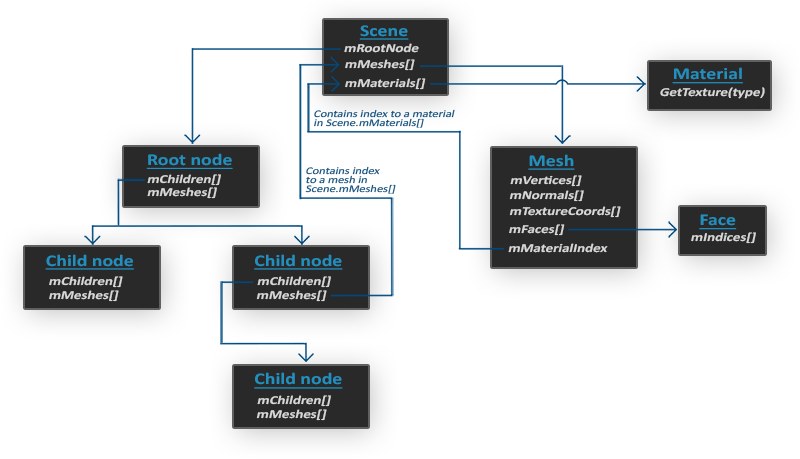
\includegraphics[width=\textwidth,height=\textheight,keepaspectratio]{Figures/Ch5/assimp_structure.png}}

	\caption{ساختار کلاس‌های کتابخانه‌ی \lr{Assimp} \cite{LearnOpenGL_Assimp}}
	\label{fig:Assimp}
  \end{figure}
  


  
\subsection{\lr{stb}}

این کتابخانه برای بارگذاری تصاویر استفاده می‌شود. در این پروژه از این کتابخانه برای بارگذاری
تصاویر بافت‌ها در کنار کتابخانه‌ی 
\lr{Assimp}
استفاده شده است.
\cite{stb}